% !Mode:: "TeX:UTF-8"

\titlepage

\begin{frame}{说在前面}
	\linespread{1.5}
	  \begin{itemize}[<+-|alert@+>]
	    \item \ba{雷同!!!}
	    \item \ba{雷同!!!}
	    \item \ba{雷同!!!}
	  \end{itemize}
\end{frame}

% \begin{frame}{需要注意的问题}
% 	\linespread{1.5}
% 	  \begin{itemize}%[<+-|alert@+>]
% 	    \item L'Hospital法则
% 	    \begin{itemize}
% 	      \item \it 只能应用于“$\df{\bm{0}}{\bm{0}}$”
% 	      和“$\df{\bm{\infty}}{\bm{\infty}}$”型
% 	      \item \it 及时使用无穷小代换进行简化
% 	      \item \it 不正规的符号:\b 
% 	      $\xlongequal{\footnotesize\mbox{“L”}}$、
% 	      $\xlongrightarrow{\footnotesize\mbox{“L'Hospital法则”}}$、
% 	      $\df{\bm{0}}{\bm{0}}$、$\df{\bm{\infty}}{\bm{\infty}}$
% 	    \end{itemize}
% 	    \item Taylor公式
% 	    \begin{itemize}
% 	      \item \it Taylor多项式不包含余项
% 	      \item \it 合并同次幂的系数
% 	      \item \it 尽量按照幂次由低到高排列,最后写余项
% 	    \end{itemize}
% 	  \end{itemize}
% \end{frame}

\section{7.3 可降阶的二阶微分方程}

\begin{frame}
	\linespread{1.5}
	\ba{1.求解下列初值问题:	
	(1)$xy''=y',y(0)=1,y'(1)=0$}
	
	\bigskip
	
	\small 解:\it
	令$p=y'$,则原方程即为
	$$xp'=p,$$
	分离变量可解得$p=Cx,\;(C\in\mbb{R})$,也即
	$$y'=Cx,$$
	从而可得
	$$y=C_1x^2+C_2,\quad (C_1,C_2\in\mbb{R}),$$
	带入初值条件可得$C_2=1,C_1=0$,故所求方程的特解为
	$$y=1.$$
\end{frame}

\begin{frame}
	\linespread{1.5}
	\ba{(2)$y''+(y')^2=1,y(0)=y'(0)=1$}
	
% 	\bigskip
	
	\small 解:\it
	令$p=y'$,则原方程即为
	$$p'+p^2=1,$$
	该方程等价于
	$$\df{\d p}{1-p^2}=\d x\;(1-p^2\ne 0)\quad
	\mbox{或}\quad p=\pm 1.$$
	注意到$p(0)=y'(0)=1$,故必有$p=y'=1$,进而可得
	$$y=x+C,$$
	又$y(0)=1$,可得$C=1$,从而所求特解为
	$$y=x+1.$$
\end{frame}

\begin{frame}
	\linespread{1.5}
	\ba{(3)$y''-y=0,y(0)=0,y'(0)=1$}
	
% 	\bigskip
	
	\small 解:\it
	令$p=y'$,则原方程化为
	$$pp'-y=0,$$
	分离变量解之可得$p=\sqrt{y^2+C_1},\;(C_1\in\mbb{R})$,也即
	$$y'=\sqrt{y^2+C_1},$$
	带入初值条件,可解得$C_1=1$,进而
	$y'=\sqrt{y^2+1}$,
	分离变量解之可得
	$$y=\df{e^{x+C_2}-e^{-(x+C_2)}}2,\quad (C_2\in\mbb{R}),$$
	带入初值条件,可得$C_2=0$,故所求方程的特解为
	$$y=\df{e^x-e^{-x}}2.$$
	\fin
\end{frame}

\begin{frame}
	\linespread{1.5}

% 	\bigskip

	\begin{columns}
		\begin{column}{.55\textwidth}
			\ba{2.已知曲线$y=y(x)$光滑、严格单调递增,且经过点$(0,1)$。
			记其上任一点$P(x,y)$处的切线与$x$轴的交点为$Q$,以$PQ$为斜边,
			$x$轴为一条直角边的直角三角形的面积为$S_1$。对应于区间$[0,x]$的
			曲线段与$x$轴之间的曲边梯形面积为$S_2$。已知$2S_1-S_2=1$,求
			曲线方程。}
		\end{column}
		\begin{column}{.4\textwidth}
			\begin{center}
				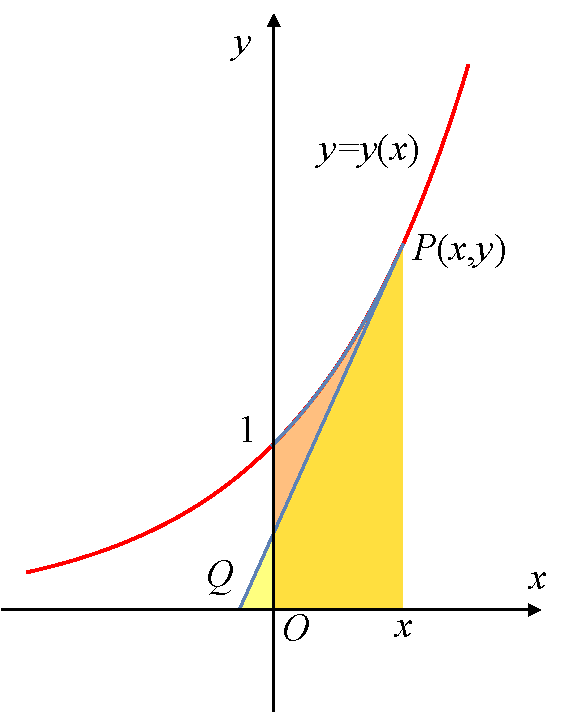
\includegraphics[width=\textwidth]{./images/ch7/eX.pdf}
			\end{center}
		\end{column}
	\end{columns}
\end{frame}

\begin{frame}
	\linespread{1.5}	
	\small 解:\it
	设所求曲线为$y=y(x)$,过其上任一点$P(x,y)\;(x\geq 0)$的切线为
	$$Y=y+y'(X-x),$$
	与$x$轴相交于$Q(x-x/y',0)$。由于$y'>0$,故当$x\geq 0$时,恒有$y\geq 1$,故
	$$S_1=\df12y\left[x-\left(x-\df{y}{y'}\right)\right]=\df{y^2}{2y'}.$$
	又
	$$S_2=\dint_0^xy(t)\d t,$$
	由已知$2S_1-S_2=1$,也即
	$$\df{y^2}{y'}-\dint_0^xy(t)\d t=1.$$
\end{frame}

\begin{frame}
	\linespread{1.5}	
	\small \it
	$$\df{y^2}{y'}-\dint_0^xy(t)\d t=1.$$
	
	对该方程两边连求导,并取$x=0$可得
	$$\left\{\begin{array}{l}
	yy''=(y')^2\\
	y(0)=1\\
	y'(0)=1
	\end{array}\right.$$
	解之得$y=e^x$,即为所求。
	\fin
\end{frame}

\section{7.4 二阶线性微分方程}

\begin{frame}
	\linespread{1.5}
	\ba{1.求解下列微分方程:(1)$y''-y=e^x+\cos x$}
	
	\bigskip
	
	\small 解:\it
	该方程的特征方程为$r^2-1=0$,特征根为$r=\pm1$,
	故其对应的齐次方程的通解为$y=C_1e^x+C_2e^{-x},(C_1,C_2\in\mbb{R})$。
	
	利用叠加原理,可以设原方程的特解为
	$$y^*=Axe^x+(B\cos x+C\sin x),$$
	带入原方程可得
	$$2Ae^x-2B\cos x-2C\sin x=e^x+\cos x,$$
	从而可得$A=\frac12,B=-\frac12,C=0$。
	综上,原方程的通解为
	$$y=C_1e^x+C_2e^{-x}+\df12xe^x-\df12\cos x,\quad (C_1,C_2\in\mbb{R})$$
\end{frame}

\begin{frame}
	\linespread{1.5}
	\ba{(2)$y^{(4)}+y''=1$}
	
	\bigskip
	
	\small 解:\it
	令$z=y''$,则原方程可化为
	$$z''+z=1,$$
	求解该方程可得其通解为$z=C_1\cos x+C_2\sin x+1,(C_1,C_2\in\mbb{R})$,
	也即
	$$y''=C_1\cos x+C_2\sin x+1,$$
	对其两边连续两次积分可得
	$$y=C_3\cos x+C_4\sin x+\df12x^2+C_5x+C_6,\quad (C_3,C_4,C_5,C_6\in\mbb{R}),$$
	即为原方程的通解。\fin
\end{frame}

\begin{frame}
	\linespread{1.5}
	\ba{2.求级数$\sumn[0]\df{x^{2n}}{(2n)!}$的和函数。 }
	
	\bigskip
	
	\small 解:\it
	该级数的收敛域为$(-\infty,+\infty)$,设其和函数为$S(x)$,则
	$$S''(x)=S(x).$$
	这是一个二阶常系数齐次线性微分方程,解之可得
	$$S(x)=C_1e^x+C_2e^{-x},\quad(C_1,C_2\in\mbb{R}).$$
	注意到$S(0)=1,S'(0)=0$,带入以上的通解,可得$C_1=C_2=\frac12$,故
	$$\sumn[0]\df{x^{2n}}{(2n)!}=\df{e^x+e^{-x}}2,\quad(x\in\mbb{R}).$$
	\fin
\end{frame}

\begin{frame}
	\linespread{1.5}
	\ba{3.设$\varphi'(x)=e^x+\sqrt x\dint_0^{\sqrt x}\varphi(\sqrt x u)\d u,$
	$\varphi(0)=0$,求$\varphi(x)$。}
	
	\bigskip
	
	\small 解:\it
	令$t=\sqrt xu$,则已知方程即为
	$$\varphi'(x)=e^x+\dint_0^x\varphi(t)\d t,$$
	对其两边关于$x$求导,结合已知条件,可得到初值问题
	$$
		\left\{\begin{array}{l}
			\varphi''(x)-\varphi(x)=e^x,\\
			\varphi(0)=0,\\
			\varphi(0)=1.
		\end{array}\right.
	$$
	解之可得
	$$\varphi(x)=\df14e^x-\df14e^{-x}+\df12xe^x.$$
	\fin
\end{frame}

\begin{frame}
	\linespread{1.5}
	\ba{4.设$y(x)$在$\mathbb{R}$上具有二阶连续导数,$y'\ne 0$,$x=x(y)$
	  为其反函数。
	    \begin{enumerate}[(1)]
% 	      \setlength{\itemindent}{1cm}
	      \item 试将$x=x(y)$所满足的微分方程
	      $$\df{\d^2x}{\d y^2}+(y+\sin x)\left(\df{\d x}{\d y}\right)^3=0$$
	      变换为$y=y(x)$所满足的微分方程;%\hfill$y''-y=-\sin x$
	      \item 求变换后的微分方程满足初始条件$y(0)=0$和$y'(0)=1.5$的解。
	    \end{enumerate}}
	
% 	\bigskip
	
% 	\small 解:\it
% 	设$m(t)$为自2000年起第$t$年时湖内的污染物总量,则
% 	$$m'=\df{m_0}6-\df{m}3,$$
% 	且$m(0)=5m_0$。
\end{frame}

\begin{frame}
	\linespread{1.5}
	\small 解:\it
	$$\df{\d^2x}{\d y^2}=\df{\d x'}{\d y}
	=\df{\d(1/y')}{\d y}=
	\df{\df{\d\frac1{y'}}{\d x}}{\df{\d y}{\d x}}=-\df{y''}{(y')^3},$$
	从而原方程可化为$y''-y=\sin x$。
	以上方程对应的齐次方程的通解为$y=C_1e^x+C_2e^{-x},(C_1,C_2\in\mbb{R})$。
	设原方程的特解为$y^*=A\cos x+B\sin x$,带入方程可解得
	$A=0,B=-\frac12$,故原方程的通解为
	$$y=C_1e^x+C_2e^{-x}-\df12\sin x,\quad (C_1,C_2\in\mbb{R}).$$
	带入初始条件,可得$C_1=-C_2=1$,故所求特解为
	$$y=e^x-e^{-x}-\df12\sin x.$$
	\fin
\end{frame}

\begin{frame}
	\linespread{1.5}
	\ba{5.设以质量为$m$的质点作直线运动。从速度等于零的时刻起,有一个与其运动方向
	一致、大小与时间成正比(比例系数为$a$)的力作用于它,与此同时地面对其的阻力
	大小与其速度成正比(比例系数为$b$),求该质点的位移函数$S(t)$(设初始位移$S(0)=0$)}
	
	\small 解:\it
	由已知
	$$S''(t)=\df{at}m-\df{bS'(t)}m.$$
	该方程对应的齐次方程的通解为$S(t)=C_1+C_2e^{-\frac{bt}m},(C_1,C_2\in\mbb{R})$。
	
	设该方程的特解为$S^*(t)=(At+B)t$,带入方程可得
	$$2A+\df bm(2At+B)=\df{at}m,$$
	由此解得$A=\df{a}{2b},B=-\df{ma}{b^2}$。
\end{frame}

\begin{frame}
	\linespread{1.5}
	
	\small \it
	
	综上原方程的通解为
	$$S(t)=C_1+C_2e^{-\frac{bt}m}+\df{at^2}{2b}-\df{mat}{b^2},
	\quad (C_1,C_2\in\mbb{R})$$
	
	又$S(0)=S'(0)=0$,带入通解中可得$C_1=\frac{m^2a}{b^3},C_2=-\frac{m^2a}{b^3}$,
	进而所求位移函数为
	$$S(x)=\frac{m^2a}{b^3}\left(1-e^{-\frac{bt}m}\right)
	+\df{at^2}{2b}-\df{mat}{b^2}.$$
	\fin
\end{frame}

% \begin{frame}{出现的问题}
% 	\linespread{1.5}
% 	  \begin{itemize}%[<+-|alert@+>]
% 	    \item 作业进度慢!
% 	    \item 概念问题
% 	    \begin{itemize}
% 	      \item \b\it 幂级数展开不熟练
% 	      \item \b\it Maclaurin级数和关于$(x-x_0)$的幂级数分不清
% 	    \end{itemize}
% 	    \item 过程不规范或不完整
% 	    \begin{itemize}
% 	      \item \b\it 求收敛域要单独讨论端点的敛散性
% 	      \item \b\it 相同幂次的项要合并,并按幂次从小到大排列
% 	      \item \b\it 书写潦草随意\pause
% 	    \end{itemize}
% 	    \item \ba{雷同!!!}
% 	  \end{itemize}
% \end{frame}

% \begin{frame}
% 	\linespread{1.5}
% 	\ba{3.设$D$是由曲线$y=\sin x+1$与三条直线$x=0,x=\pi,y=0$
% 	所围成的曲边梯形,求$D$绕$x$轴旋转一周所围成的旋转体的体积。
% 	}
% 	\pause
% 	
% % 	\bigskip
% 	
% 	\begin{columns}
% 		\begin{column}{.5\textwidth}
% 			\begin{center}
% 				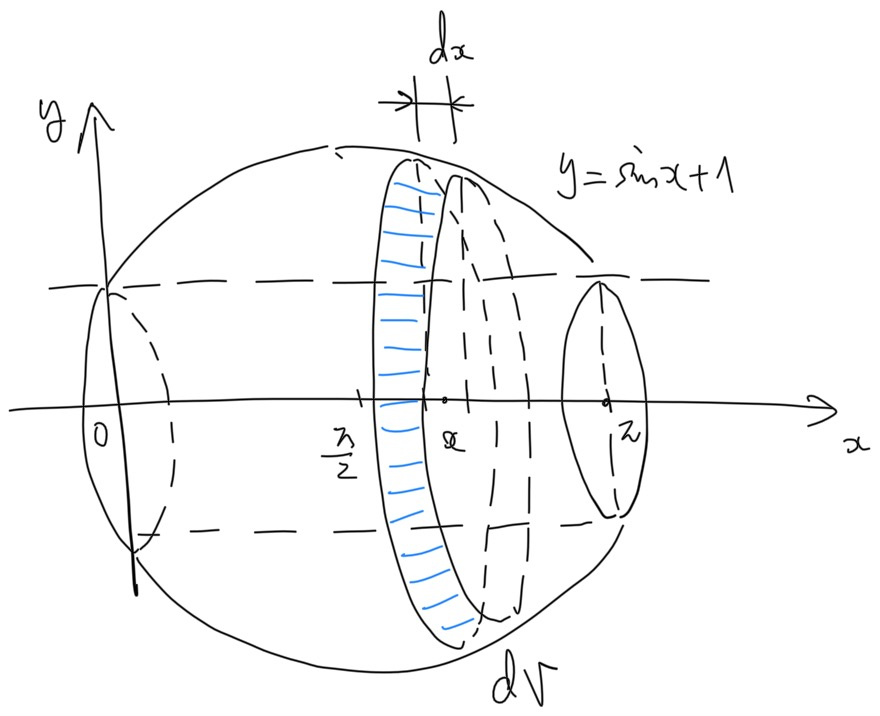
\includegraphics[width=.9\textwidth]{./images/ch6/sinx1cs.jpg}
% 		% 		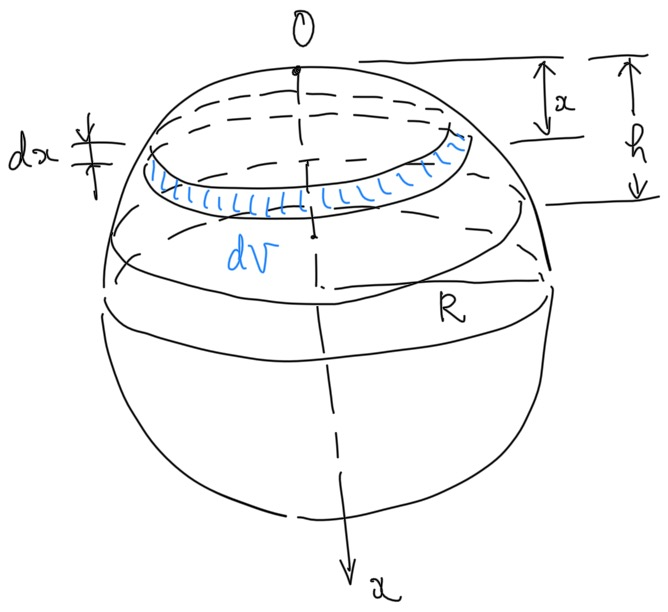
\includegraphics[width=6cm]{./images/ch6/topSp.jpg}
% 			\end{center}		
% 		\end{column}
% 		\begin{column}{.5\textwidth}
% 			\small 解:\it
% 			如图,体积微元$\d V=\pi y^2\d x$,	故所求体积
% 			$$
% 				V=\dint_0^{\pi}\pi(\sin x+1)^2\d x=\df32\pi^2.
% 			$$
% 		\end{column}
% 	\end{columns}
% \end{frame}